The "Wow!" signal seen in 1977 \citep{wow} remains the most tantalizing unexplained radio signal to this day, although many have tried to disentangle its origins (i.e. \citealt{Wow_2024}).  This signal, rendered as ``6EQUJ5'' in the observatory printout, was clearly detected and conformed to the expected sidereal signal through the telescope beam.  In today's world, it would likely have never been readily discovered since our own technological signals permeate the sky. At the time however the world didn't have so many transmitters on people, in the air, or in the heavens above.  Given all of this, the signal remains tantalizing to this day. Since it was only seen once, no conclusive evidence has been provided of its origin, which could have been anthropogenic or something more. Imagine going to a place where literally everything seen is of scientific interest and being able to explore it using modern technology that is far more advanced than the telescope used in 1977.   That is the promise of a lunar farside telescope.

Humanity is at a tipping point for conducting effective radio astronomical observations from Earth. The ever-increasing use of wireless communication devices on the ground and in orbit means that nowhere on our planet, even remote locations with very low population density, is free of significant radio frequency interference (RFI). We have already gone to space with a small number of very expensive ``Great Observatories'', but the advent of accessible and relatively cost-effective access to space means that deploying a larger number of smaller telescopes is now feasible. We are therefore at the tip of the spear of the transition from earth-based to space-based telescopes for radio astronomy --- born of necessity to respond to changes in Earth’s RF environment\footnote{Note that other wavelengths have always needed or at least prefered to be above the atmosphere due to absoprtion and scattering by atmospheric constituents.}; observations above the Earth's atmposphere and ionosphere also open up an observing window inaccesible from Earth.

While terrestrial wireless communications only have negative implications for radio astronomy observations, the same technology drivers for cost-effective access to space means that smaller telescopes and experiments may be deployed to places with significantly less RFI. As this change happens, the associated electronics, along with other active transmitters in space will begin injecting RFI into those domains. This makes it urgent to get well-designed sensors into space as soon as possible to make early baseline measurements and conduct the unique science allowed by the current environment which benefits from a complete lack of RFI. The lunar farside is unique in our solar system in that it always has its back turned to the Earth \citep{MACCONE2019233,michaud2020lunar,heidmann2002}. The lunar farside currently presents a once-in-human-history opportunity to record signals in a fully quiet environment. However this is for a limited time opportunity given the great interest of deploying assets in and around the moon, as seen in Fig. \ref{fig:missions}.

\begin{figure}
    \centering
    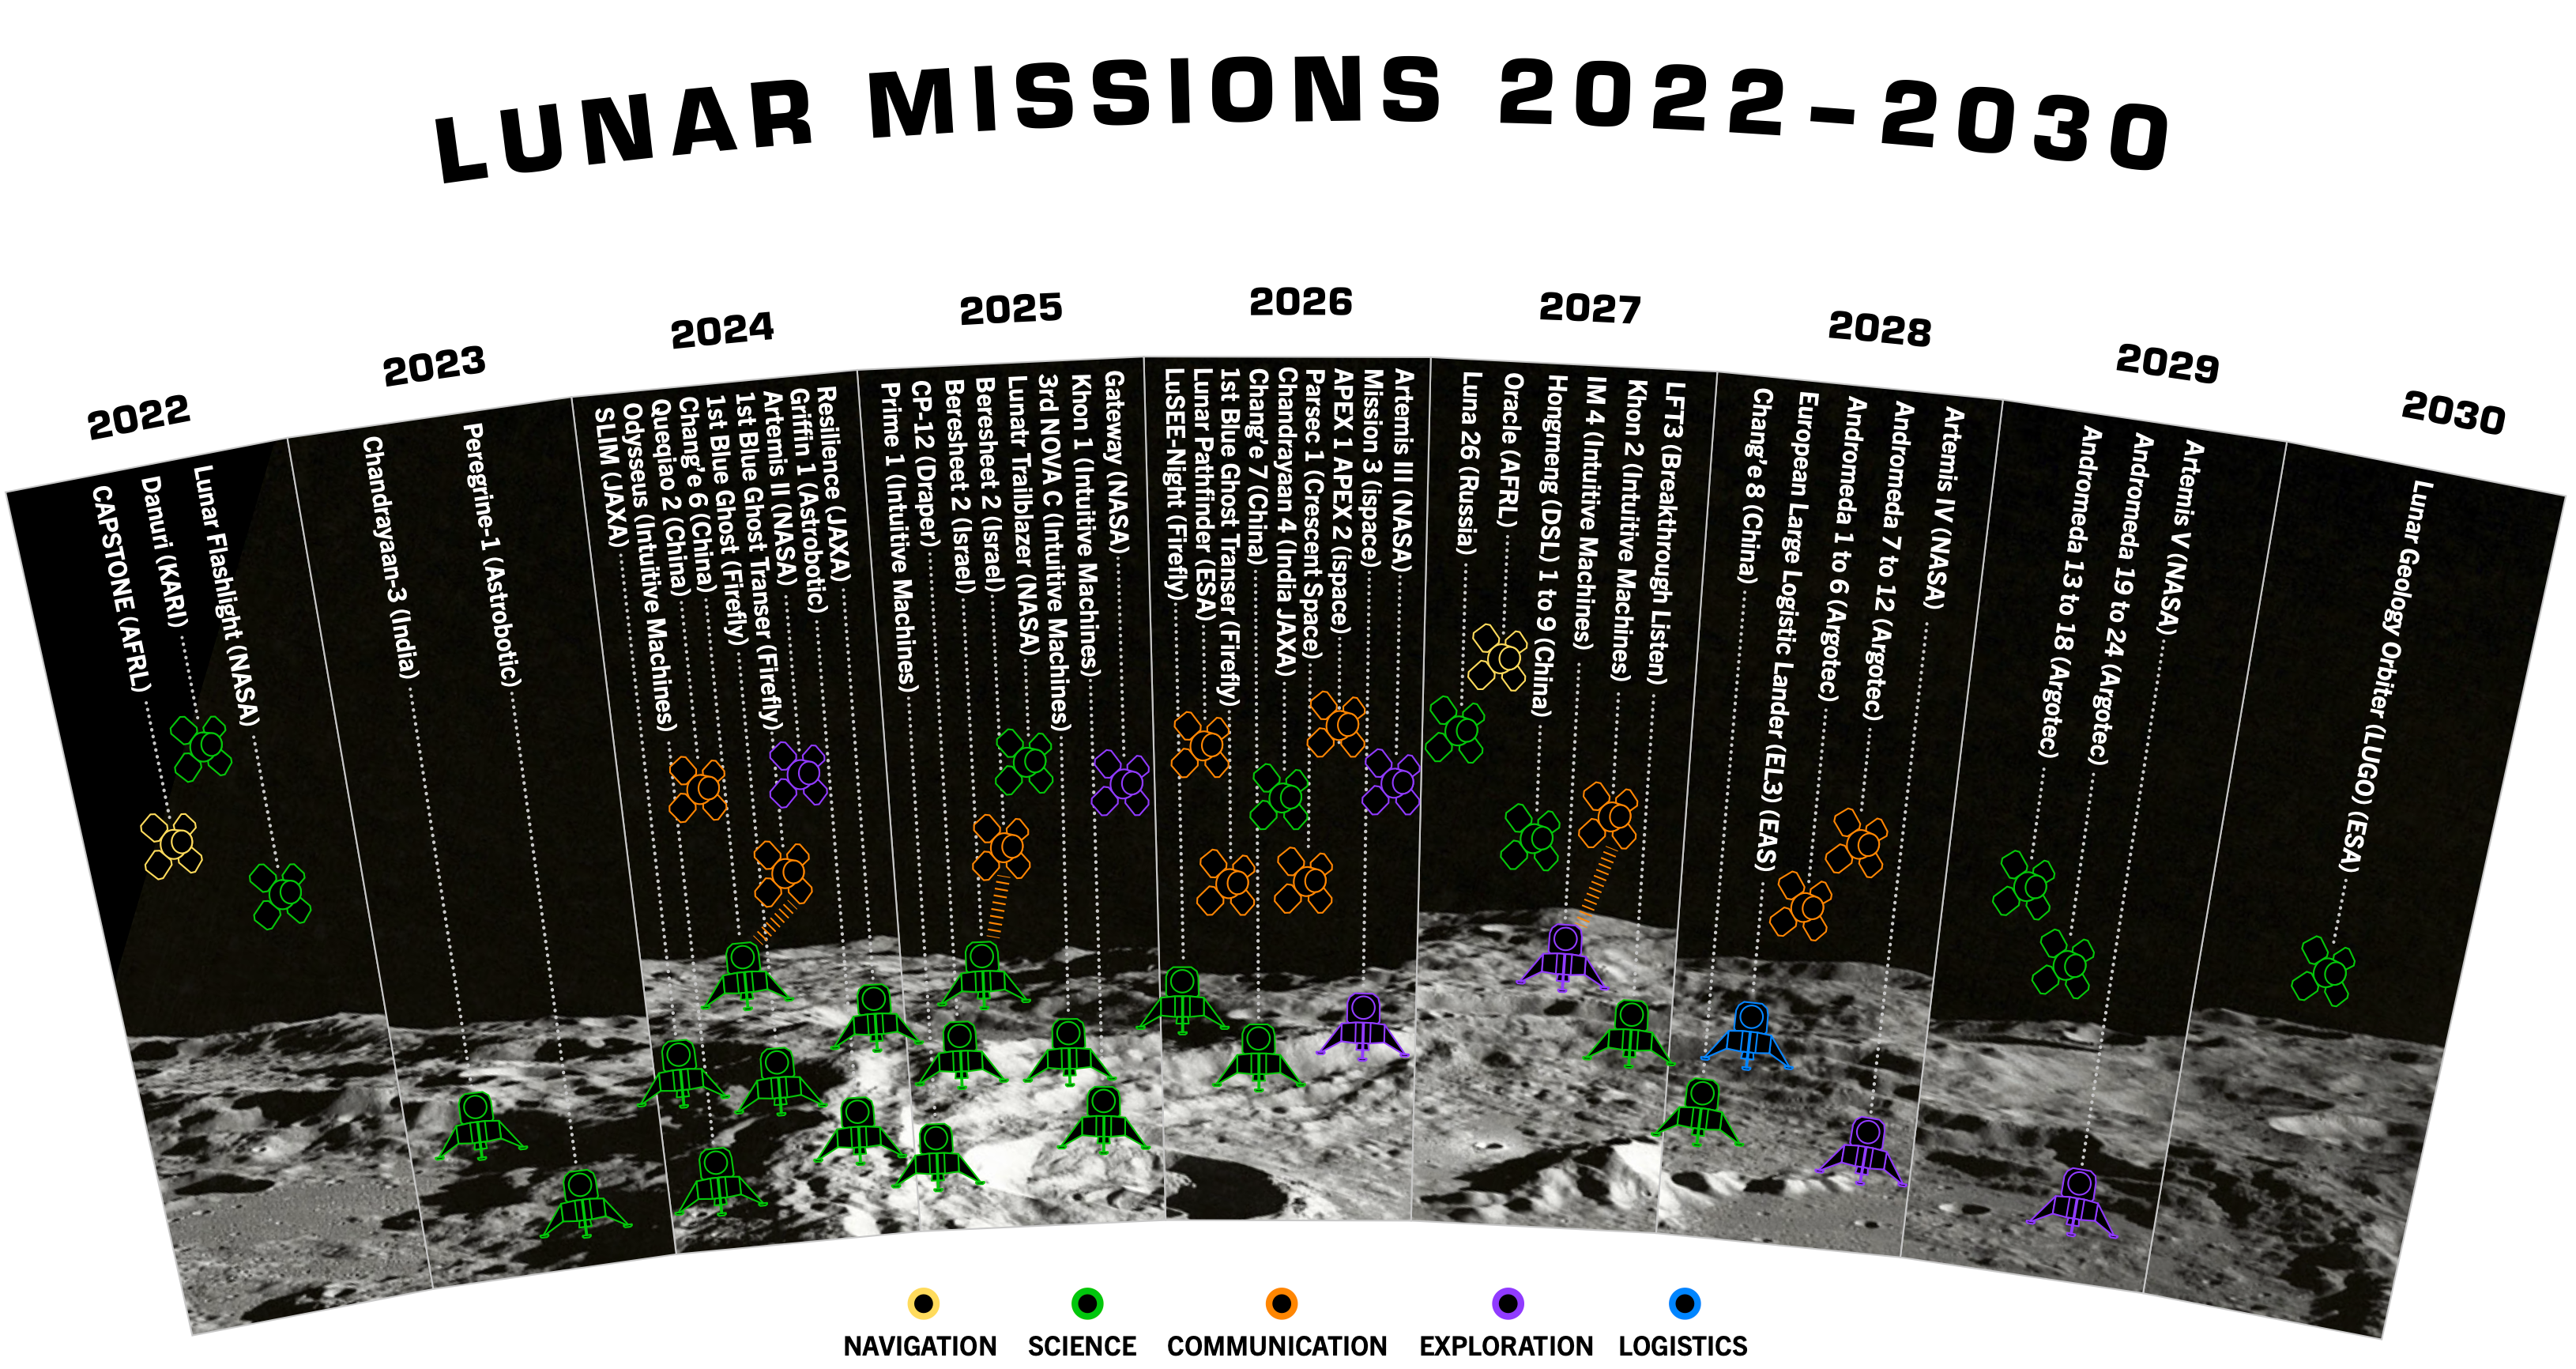
\includegraphics[width=0.95\linewidth]{figures/missions.png}
    \caption{Graphic showing the planned upcoming cislunar missions.}
    \label{fig:missions}
\end{figure}

To act on this singular opportunity, we propose a radio telescope to be landed near the lunar antipode within five years to conduct these unique-in-history measurements. The telescope will comprise of UHF dual-pol multibeam phased array operating from $300-900$~MHz as well as individual antennas to receive $1-50$~MHz, $60-110$~MHz and $900-2700$~MHz. Figure \ref{fig:freqbands} shows the frequency bands and their sensitivity.  During its mission lifetime, the telescope will observe most of the sky (see Fig. \ref{fig:fieldofview}) and conduct historical surveys in the most RFI-pristine environment in the solar system before humanities presence increases the radio frequency interference, even at this very remote place.  By the end of the decade it is likely that more than a dozen spacecraft will be orbiting the moon.

\begin{figure}
    \centering
    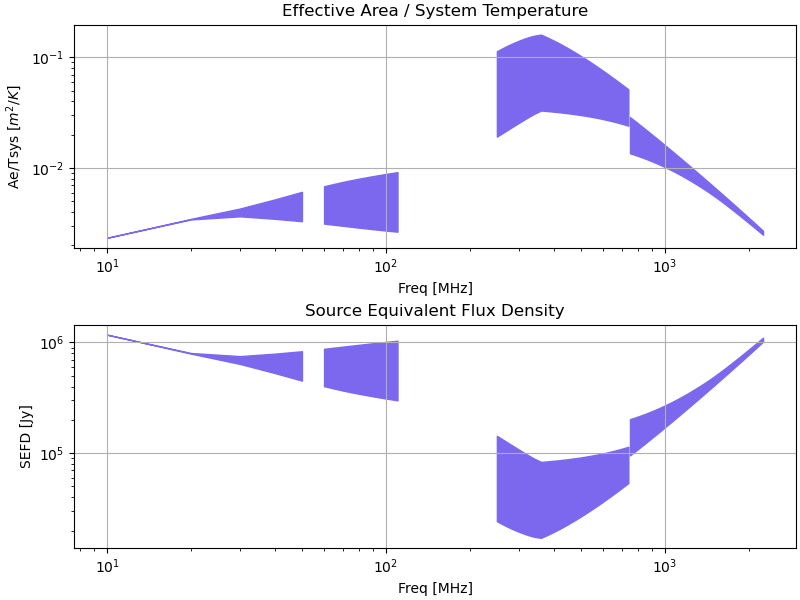
\includegraphics[width=0.75\linewidth]{figures/freqbands.png}
    \caption{Frequency bands of LFT3 and their associated ranges in sensitivity in terms of effective area over system temperature (top) and source equivalent flux density (bottom). The range stems from the varying sky temperatures.}
    \label{fig:freqbands}
\end{figure}

\begin{figure}
    \centering
    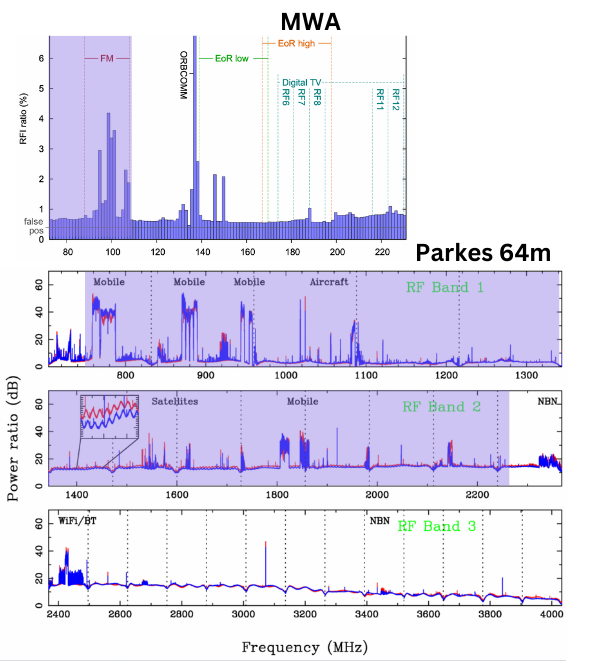
\includegraphics[width=0.75\linewidth]{figures/RFI_Plot.png}
    \caption{Figure showing the RFI environment at the Murchison Widefield Array (MWA; \citealt{Offringa_RFI}) and the Parkes 64m \citep{Hobbs_2020} telescopes. Highlighted are the regions proposed for use by the lunar telescope. }
    \label{fig:RFI}
\end{figure}

In addition to RFI considerations, which can be extensive as shown in Figure \ref{fig:RFI}, there are other scientific reasons for locating a radio telescope on the moon. The ionosphere surrounding our planet creates a conducting medium through which
%NEED TO CLEAN UP REMAINDER OF PARAGRAPH
electromagnetic radiation can't clearly pass through. Although this will not have a significant effect on observations above 1\,GHz, the lower frequencies are impacted as a wavelength squared relationship. Therefore, as we head toward meter wavelengths, we are impacted by shifting of the source position and potential for plasma screens making the sky opaque. Ground-based observations become infeasible after a frequency cutoff of 10--30\,MHz. Due to the absence of an ionosphere on the moon, there are no technical barriers to studying physics at these new frequencies.

When considering this endeavor, the following factors should be considered:

\begin{itemize}
    \item At low frequencies the system temperature will be dominated by Galactic noise and impulsive events will be affected by scattering. Any civilization generating a beacon will be aware of this constraint regardless of where they are located in the Galaxy and tends to discourage arguments for low-frequency SETI.  However, this is an unexplored region of frequency space and should be thorougly observed;
    \item Having the widest possible absolute bandwidth and largest feasible field-of-view will maximize the possibility for serendipitous discoveries;
    \item The possibility of initial discovery of technosignatures in the aforementioned bands with Earth-based telescopes is drowned out by ``anthropogenic technosignatures” aka RFI.  The lunar farside should be completely devoid of this for at least 5 years;
   \item LuSEE-Night will operate from the lunar farside at radio frequencies (0.1-50MHz) that are below the Earth's ionospheric cutoff to make radio astronomical observations impossible, which can be augmented by this telescope;
    \item An all-sky monitor from the lunar surface will give an unprecedented view of bright, but rare transient events, including those obscured by the atmosphere and RFI from the earth.
\end{itemize}

We note that an observatory on the far-side of the moon has no visibility of Earth, and thus would have limited use for defense/intelligence purposes, emphasizing its peaceful, scientific-use only purpose. Potential science cases for bringing this telescope to life are outlined in the next section followed by a discussion of the payload and operational model.